\section{Problem 2}

{\bfseries 2.1 Part 1}

\begin{figure}[!htb]
\minipage{0.24\textwidth}
  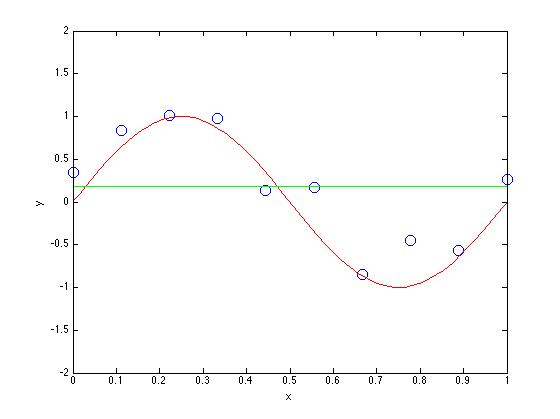
\includegraphics[width=\linewidth]{figures/p2_MLE_M=0}
  \caption{M = 0}\label{fig:figures/p2_MLE_M=0}
\endminipage\hfill
\minipage{0.24\textwidth}
  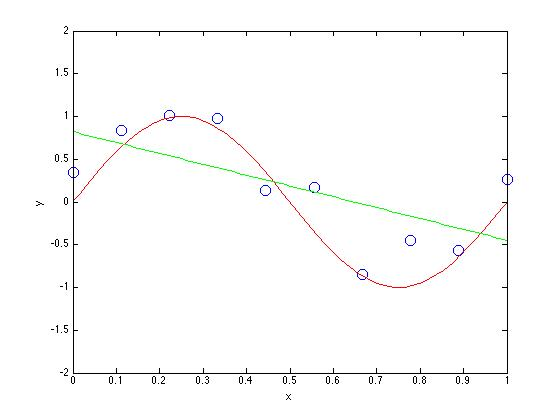
\includegraphics[width=\linewidth]{figures/p2_MLE_M=1}
  \caption{M = 1}\label{fig:figures/p2_M=1}
\endminipage\hfill
\minipage{0.24\textwidth}                                                                            
  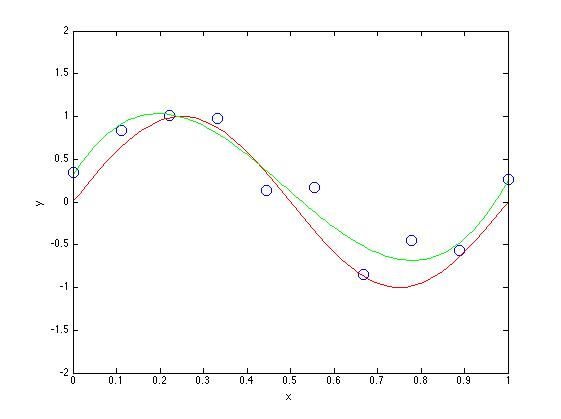
\includegraphics[width=\linewidth]{figures/p2_MLE_M=3}
  \caption{M = 3}\label{fig:figures/p2_M=3}
\endminipage\hfill
\minipage{0.24\textwidth}                                                                            
  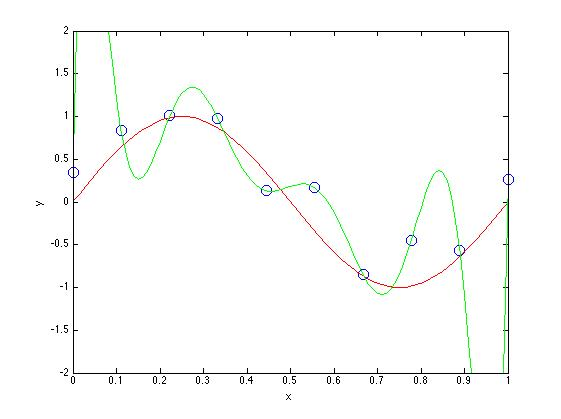
\includegraphics[width=\linewidth]{figures/p2_MLE_M=9}
  \caption{M = 9}\label{fig:figures/p2_M=9}
\endminipage\hfill
\end{figure}

We first computed the maximum likelihood weight vector and replicated 
the Bishop Figure 1.4.


{\bfseries 2.2 Part 2}

We implemented the SSE computation function and the function to compute its derivative following the formulas outlined in the handout (not listed here due to space contraints.)
We tested a few data points using numerical gradient and analytical gradient for each function.
The error we observed is small for smaller Ms (M = 2 and 3).  We used the same precision explained
 in part 3 of problem 1. For the 10 data points we chose, the gradient we calculated using analytical and numerical approaches are the same to the 4th decimal places. The numerical method is less precise for larger M. 

{\bfseries 2.3 Part 3}
\begin{figure}[!htb]
\minipage{0.24\textwidth}
  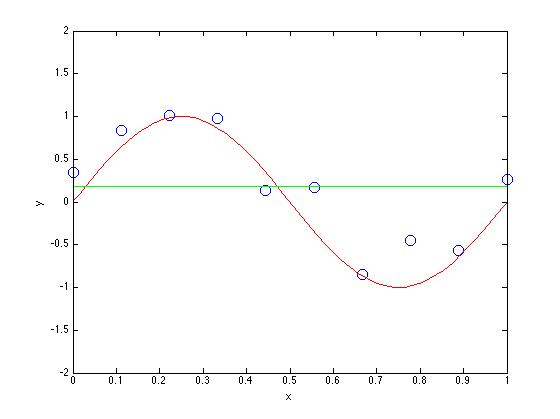
\includegraphics[width=\linewidth]{figures/p2_M=0}
  \caption{M = 0}\label{fig:figures/p2_M=0}
\endminipage\hfill
\minipage{0.24\textwidth}
  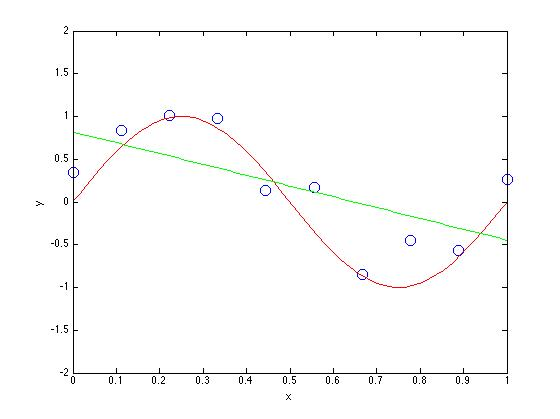
\includegraphics[width=\linewidth]{figures/p2_M=1}
  \caption{M = 1}\label{fig:figures/p2_M=1}
\endminipage\hfill
\minipage{0.24\textwidth}                                                                            
  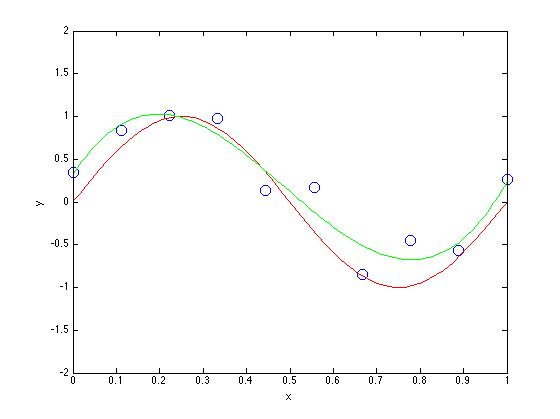
\includegraphics[width=\linewidth]{figures/p2_M=3}
  \caption{M = 3}\label{fig:figures/p2_M=3}
\endminipage\hfill
\minipage{0.24\textwidth}                                                                            
  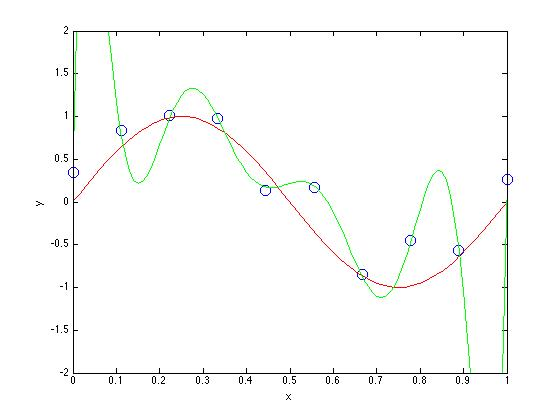
\includegraphics[width=\linewidth]{figures/p2_M=9}
  \caption{M = 9}\label{fig:figures/p2_M=9}
\endminipage\hfill
\end{figure}


We used gradient descent to replicate 
the Bishop Figure 1.4 and verified the paramteres in the same way in part1. 
\textit{Convergence criteria:} we generally chose the threshold to be around $10^{-6}$ as a convergence criteria. We selected this convergence criteria baed the on comparing the weight generated and those listed in Bishop's book and visual verification. 
\textit{Step size:} For M = 0,1,3, it is easy to use gradient descent to find the minimum of the graph. We can use larger step sizes for smaller Ms, such as 0.05. For M = 9, we had to select a smaller step size around 0.02 - 0.03. If we select a step size that is too large, we will not converge. This is because the gradient changes more quickly for larger M using SSE.
\textit{Starting guess:} The starting guess is also very important for M = 9 to converge. If we start from a point that is far from the minimum, gradient descent can take a very long time to converge or stuck at a local minimum. As a result, to generate the graph for M = 9, we had to select a starting point that is not too far from the optimial weights (We chose 1.1 magnitude difference for the dimensions). This is because for large M, the weight for SSE can often be very large positive or negative numbers. 
\textit{optimizers:} The optimizers in Matlab (fminunc) uses much fewer iterations than our own gradient descent. For M = 1, our gradient descent uses 153 iterations and fminunc uses 8 iterations. (for M = 9, our gradient descent uses 1000x more iterations than fminunc). We believe fminunc doesn't use a fixed step size and implemented other optimizations. 
